%[John's picture]

\begin{center}
\resizebox{1\textwidth}{!}{%
\trimbox{0cm 0cm 1.5cm 0cm}{ 
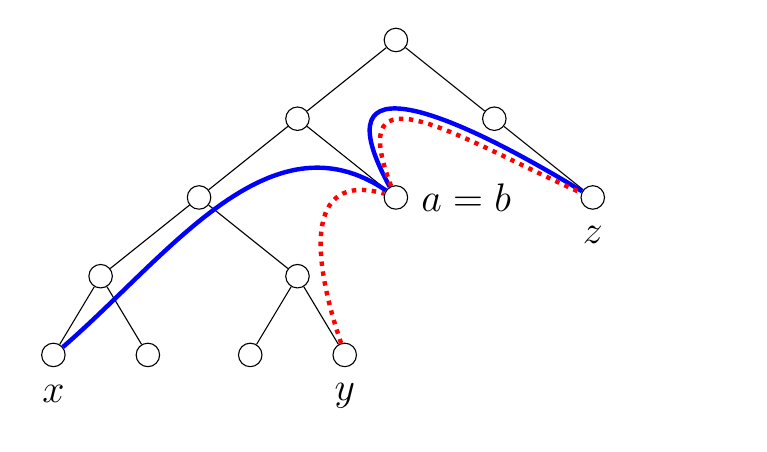
\begin{tikzpicture}[level distance=10mm, state/.style={circle, draw, minimum size=1mm}]]
  \tikzstyle{every node}=[font=\Large, draw=black, circle,inner sep=3pt]
  \tikzstyle{level 1}=[sibling distance=25mm, set style={{every node}+=[draw=black]}]
  \tikzstyle{level 2}=[sibling distance=25mm, set style={{every node}+=[draw=black]}]
  \tikzstyle{level 3}=[sibling distance=25mm,  set style={{every node}+=[draw=black]}]
  \tikzstyle{level 4}=[sibling distance=12mm,  set style={{every node}+=[draw=black]}]
  \tikzstyle{level 5}=[sibling distance=5mm,  set style={{every node}+=[draw=black]}]

  \node (1) {}
     child {node (2) {}
      child {node (3) {}
       child {node (4) {}
        child {node[label=below:{$x$}] (x) {}}
        child {node (5) {}}
       }
       child {node (6) {}
        child {node (7) {}}
        child {node[label=below:{$y$}] (y) {}}
       }
      }
      child {node[label=right:{$a=b$}] (a) {}
       child[fill=none] {edge from parent[draw=none]
        child[fill=none] {edge from parent[draw=none]}
        child[fill=none] {edge from parent[draw=none]}
        }
       child[fill=none] {edge from parent[draw=none]
        child[fill=none] {edge from parent[draw=none]}
        child[fill=none] {edge from parent[draw=none]}
       }
      }
      }
      child {node (9) {}
       child[fill=none] {edge from parent[draw=none]
        child[fill=none] {edge from parent[draw=none]
         child[fill=none] {edge from parent[draw=none]}
         child[fill=none] {edge from parent[draw=none]}
         }
       child[fill=none] {edge from parent[draw=none]
        child[fill=none] {edge from parent[draw=none]}
        child[fill=none] {edge from parent[draw=none]}
       }
      }
       child {node[label=below:{$z$}] (z) {}
        child[fill=none] {edge from parent[draw=none]
         child[fill=none] {edge from parent[draw=none]}
         child[fill=none] {edge from parent[draw=none]}
        }
       child[fill=none] {edge from parent[draw=none]
        child[fill=none] {edge from parent[draw=none]}
        child[fill=none] {edge from parent[draw=none]}
        }
       }
       };

       \draw[-, solid,ultra thick,relative,blue] (x) to[out=15,in=120, looseness=1] (a);

       \draw[-, solid,ultra thick,relative,blue] (a) to[out=120,in=150, looseness=2] (z);

       %out=120,in=150, looseness=2
       %out=113,in=158, looseness=1.8

       \draw[-, dotted,ultra thick,relative,red] (y) to[out=35,in=90, looseness=1.4] (a);

       \draw[-, dotted,ultra thick,relative,red] (a) to[out=113,in=158, looseness=1.8] (z);
       

\end{tikzpicture}
}
}
\end{center}